\documentclass{article}
\usepackage{graphicx}
\usepackage{listings}
\usepackage{xcolor}
\usepackage{tcolorbox}
\usepackage{tikz}
\usepackage{amsmath}

\newcommand{\loss}{\mathcal{L}oss}

\lstdefinestyle{mystyle}{
    language=Python,
    basicstyle=\small\ttfamily,
    keywordstyle=\color{blue},
    stringstyle=\color{red},
    commentstyle=\color{green},
    breaklines=true,
    showstringspaces=false,
    frame=tb,
    backgroundcolor=\color{gray!10},
}

\title{ML\_HW4}
\author{Javad Kavian\\810100103}
\date{\today}

\begin{document}
\maketitle

\section*{Question 1}

\subsection*{A}
There are several reasons for which we use activation functions in neural networks:
\begin{enumerate}
\item Introducing non linearity to model:No matter how much we increase depth of the network, all the neurons do linear operations and if we don't add non linearity using activation functions, the model will not be able to represent non linear data

\item Introducing Sparsity: Some activation functions, like ReLU, introduce sparsity in the network by setting negative values to zero. This can lead to more efficient representations and faster computations, as only a subset of neurons are active at any given time.

\item Biological Inspiration: Many activation functions are inspired by biological neurons. For example, the sigmoid function mimics the firing rate of a biological neuron, providing a smooth transition between different activation states.
\end{enumerate}


\subsection*{B}
The problem of sigmoid activation function is the problem of vanishing gradients.The value of sigmoid function changes very smoothly in very high or very short value and thus the gradients are close to zero which which leads to slow convergence of the model.One activation function which can solve this problem is the \textbf{ReLU} activation function which only activates for positive inputs which helps to prevent the vanishing of the gradients.

\subsection*{C}
As we can see, classes can be seperated with two lines;thus we can use two neoruns to in the hidden layer to figure out whether the samples are located under the line or above it using \textbf{step} activation function and finally use a neuron in the output layer to distinguish the class analyzing the position of samples with respect to the two lines mentioned earlier:

\includegraphics[width = \textwidth]{1.png}

\includegraphics[width = \textwidth]{2.png}


and finally the output neorun can simply add the output of the two neurons of the hidden layer with $weight = 1$ and add it with a $bias = 1$ to get the index of the class of the data
    

\subsection*{C}
As we see, the function is constructed of two lines;thus we need two hidden layers.the first layer simply infers whether the input is less than $\frac{1}{3}$ or not and the second layer constructs the lines.The calculated weights and bias are as follows:

\includegraphics[width = \textwidth]{3.png}

and with the following python code, we can verify its truthness:

\begin{lstlisting}[style=mystyle]
    import numpy as np
    import matplotlib.pyplot as plt
    def ReLU(x):
        return np.maximum(x, 0)

    def N1(x):
        return ReLU(x-1/3)


    def N2(x):
        return ReLU(-x + 1/3)

    def N3(n1, n2):
        return ReLU((-3/2)*n1 + 1)

    def N4(n1, n2):
        return ReLU(-3*n2 + 1)

    def N5(n3, n4):
        return ReLU(n3+n4 - 1)

    x = np.linspace(0, 1, 100)
    n1 = N1(x)
    n2 = N2(x)
    n3 = N3(n1, n2)
    n4 = N4(n1, n2)
    y = N5(n3, n4)

    plt.plot(x, y)
    plt.grid()
    plt.show()


    
\end{lstlisting}

which gives as output the following figure:

\includegraphics[width = \textwidth]{4.png}

\subsection*{D}
An MLP with one hidden layer and a summing output unit can generate a square pulse:

\includegraphics[width = \textwidth]{5.png}

We can divide any arbitrary continous function to many number of square pulses: 

\includegraphics[width = \textwidth]{6.png}

and we can model each of these square pulses with the MLP unit shown in figure.The final MLP would be something like:

\includegraphics[width = \textwidth]{7.png}

\section*{Question 2}
In the following network, we first do a forward pass to calculate the error and then do the back propagation:

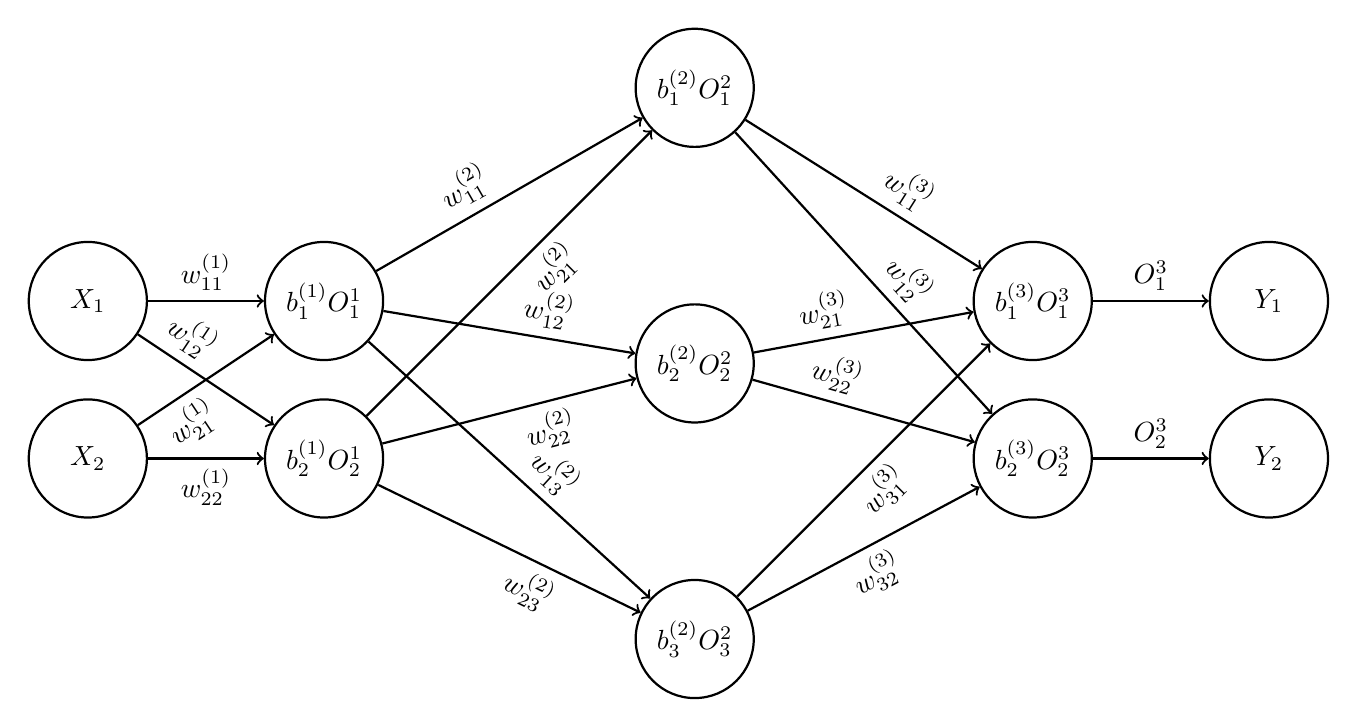
\begin{tikzpicture}[thick, main/.style = {draw, circle, minimum size=1.5cm}]
    \node[main] (1) {$X_{1}$};
    \node[main] (2) [below of=1, yshift=-1cm] {$X_{2}$};
    \node[main] (3) [right of=1, xshift=2cm] {$b_{1}^{(1)} \\ O_{1}^{1}$};
    \node[main] (4) [right of=2, xshift=2cm] {$b_{2}^{(1)} \\ O_{2}^{1}$};
    \node[main] (5) [above right of = 3, xshift=4cm, yshift = 2cm] {$b_{1}^{(2)} \\ O_{1}^{2}$};
    \node[main] (6) [below of=5, yshift = -2.5cm] {$b_{2}^{(2)} \\ O_{2}^{2}$};
    \node[main] (7) [below of=6, yshift=-2.5cm] {$b_{3}^{(2)} \\ O_{3}^{2}$};
    \node[main] (8) [right of=3, xshift=8cm]{$b_{1}^{(3)} \\ O_{1}^{3}$};
    \node[main] (9) [right of=4, xshift=8cm]{$b_{2}^{(3)} \\ O_{2}^{3}$};
    \node[main] (10) [right of=8, xshift=2cm]{$Y_{1}$};
    \node[main] (11) [right of=9, xshift=2cm]{$Y_{2}$};

    % \draw[->](1) -- node[right]{+1}(2);
    \draw[->](1) --node[above]{$w_{11}^{(1)}$}(3);
    \draw[->](1) --node[above left,sloped]{$w_{12}^{(1)}$}(4);
    \draw[->](2) --node[below left, sloped]{$w_{21}^{(1)}$}(3);
    \draw[->](2) --node[below]{$w_{22}^{(1)}$}(4);
    \draw[->](3) --node[above left, sloped]{$w_{11}^{(2)}$}(5);
    \draw[->](3) --node[above right, sloped]{$w_{12}^{(2)}$}(6);
    \draw[->](3) --node[above right, sloped]{$w_{13}^{(2)}$}(7);
    \draw[->](4) --node[below right, sloped]{$w_{21}^{(2)}$}(5);
    \draw[->](4) --node[below right, sloped]{$w_{22}^{(2)}$}(6);
    \draw[->](4) --node[below right, sloped]{$w_{23}^{(2)}$}(7);
    \draw[->](5) --node[above right, sloped]{$w_{11}^{(3)}$}(8);
    \draw[->](5) --node[above right, sloped]{$w_{12}^{(3)}$}(9);
    \draw[->](6) --node[above left, sloped]{$w_{21}^{(3)}$}(8);
    \draw[->](6) --node[above left, sloped]{$w_{22}^{(3)}$}(9);
    \draw[->](7) --node[below, sloped]{$w_{31}^{(3)}$}(8);   
    \draw[->](7) --node[below, sloped]{$w_{32}^{(3)}$}(9);   
    \draw[->](8) --node[above]{$O_{1}^{3}$}(10);
    \draw[->](9) --node[above]{$O_{2}^{3}$}(11);
    
\end{tikzpicture}

\subsection*{Forward}
\subsubsection*{Layer 1}
\begin{equation*}
    O_{1}^{1} = \frac{1}{1 + e^{-(X_{1}w_{11}^{(1)} + X_{2}w_{21}^{(1)} + b_{1}^{(1)})}}
\end{equation*}
\begin{equation*}
    O_{2}^{1} = \frac{1}{1+e^{-(X_{1}w_{12}^{(1)} + X_{2}w_{22}^{(1)} + b_{2}^{(1)})}}
\end{equation*}
\
\subsubsection*{Layer 2}

\begin{equation*}
    O_{1}^{2} = \frac{1}{1 + e^{-(O_{1}^{1}w_{11}^{(2)} + O_{2}^{1}w_{21}^{(2)} + b_{1}^{(2)})}}    
\end{equation*}

\begin{equation*}
    O_{2}^{2} = \frac{1}{1 + e^{-(O_{1}^{1}w_{12}^{(2)} +O_{2}^{1}w_{22}^{(2)}+b_{2}^{(2)})}}
\end{equation*}

\begin{equation*}
    O_{3}^{2} = \frac{1}{
        1 + e^{-(
            O_{1}^{1}w_{13}^{(2)}+
            O_{2}^{1}w_{23}^{(2)}+
            b_{3}^{(2)}
        )}
    }
\end{equation*}

\subsubsection*{Layer 3}
\begin{equation*}
    z_{1} = O_{1}^{2}w_{11}^{(3)} + O_{2}^{2}w_{21}^{(3)} + O_{3}^{2}w_{31}^{(3)} + b_{1}^{(3)}
\end{equation*}

\begin{equation*}
    z_{2} = O_{1}^{2}w_{12}^{(3)} + O_{2}^{2}w_{22}^{(3)} + O_{3}^{2}w_{32}^{(3)} + b_{2}^{(3)}
\end{equation*}

\begin{equation*}
    O_{1}^{3} = \frac{e^{z_{1}}}{e^{z_{1}} + e^{z_{2}}}
\end{equation*}

\begin{equation*}
    O_{2}^{3} = \frac{e^{z_{2}}}{e^{z_{1}} + e^{z_{2}}}
\end{equation*}

\subsubsection*{Loss Calculation}
Here we are using cross entropy loss which is formulated as below in this example:

\begin{equation*}
    \mathcal{L}oss = Y_{1}\log{O_{1}^{3}} + Y_{2}\log{O_{2}^{3}}
\end{equation*}

\subsection*{Back Propagation}
We start calculating the derivative of loss with respect to output of layers and using chaing rule, go back untill we reach the first layer:

\begin{equation}
    \frac{\partial{\loss}}{\partial{O_{1}^{3}}} = \frac{Y_{1}}{O_{1}^{3}}
\end{equation}
    
\begin{equation}
    \frac{\partial{\loss}}{\partial{O_{2}^{3}}} = \frac{Y_{2}}{O_{2}^{3}}
\end{equation}

\begin{equation}
    \frac{\partial{\loss}}{\partial{z_{1}}} = \frac{\partial{\loss}}{\partial{O_{1}^{3}}}\frac{\partial{O_{1}^{3}}}{\partial{z_{1}}} = \frac{Y_{1}}{O_{1}^{3}}
    \frac{e^{z_{1} + z_{2}}}{(e^{z_{1}} + e^{z_{2}})^2}
\end{equation}
    
\begin{equation}
    \frac{\partial{\loss}}{\partial{z_{2}}} = \frac{\partial{\loss}}{\partial{O_{2}^{3}}}\frac{\partial{O_{2}^{3}}}{\partial{z_{2}}} = \frac{Y_{2}}{O_{2}^{3}}
    \frac{e^{z_{1} + z_{2}}}{(e^{z_{1}} + e^{z_{2}})^2}
\end{equation}

\begin{equation*}
    \frac{\partial{\loss}}{\partial{O_{1}^{2}}} = \frac{\partial{\loss}}{\partial{z_{1}}}\frac{\partial{z_{1}}}{\partial{O_{1}^{2}}}
    + \frac{\partial{\loss}}{\partial{z_{2}}}\frac{\partial{z_{2}}}{\partial{O_{1}^{2}}}
\end{equation*}

\begin{equation}
    = \frac{\partial{\loss}}{\partial{z_{1}}}w_{11}^{(3)} + \frac{\partial{\loss}}{\partial{z_{2}}}w_{12}^{(3)}
\end{equation}

and with the same method, we have:

\begin{equation}
    \frac{\partial{\loss}}{\partial{O_{2}^{2}}} = \frac{\partial{\loss}}{\partial{z_{1}}}w_{21}^{(3)} + \frac{\partial{\loss}}{\partial{z_{2}}}w_{22}^{(3)}
\end{equation}

\begin{equation}
    \frac{\partial{\loss}}{\partial{O_{3}^{2}}} = \frac{\partial{\loss}}{\partial{z_{1}}}w_{31}^{(3)} + \frac{\partial{\loss}}{\partial{z_{2}}}w_{32}^{(3)}
\end{equation}

we have already calcualted the value of $\frac{\partial{\loss}}{\partial{z_{1}}}$ and $\frac{\partial{\loss}}{\partial{z_{2}}}$ in equations (3) and (4).Now lets move one layer back:
\begin{equation*}
    \frac{\partial{\loss}}{\partial{O_{1}^{1}}} = \frac{\partial{\loss}}{\partial{O_{1}^{2}}}\frac{\partial{O_{1}^{2}}}{\partial{O_{1}^{1}}}
    + \frac{\partial{\loss}}{\partial{O_{2}^{2}}}\frac{\partial{O_{2}^{2}}}{\partial{O_{1}^{1}}}
    + \frac{\partial{\loss}}{\partial{O_{3}^{2}}}\frac{\partial{O_{3}^{2}}}{\partial{O_{1}^{1}}}
\end{equation*}

$\frac{\partial{\loss}}{\partial{O_{1}^{2}}}$, $\frac{\partial{\loss}}{\partial{O_{2}^{2}}}$ and $\frac{\partial{\loss}}{\partial{O_{3}^{2}}}$ can be obtained from equations (5), (6) and (7).The other derivative terms have sigmoid form whose derivative looks like : $g(z)(1 - g(z))$.thus the above equation can be wrriten as:

\begin{equation}
    \frac{\partial{\loss}}{\partial{O_{1}^{1}}} = \frac{\partial{\loss}}{\partial{O_{1}^{2}}}(w_{11}^{(2)}O_{1}^{2}(1 - O_{1}^{2}))
    + \frac{\partial{\loss}}{\partial{O_{2}^{2}}}(w_{12}^{(2)}O_{2}^{2}(1 - O_{2}^{2}))
    + \frac{\partial{\loss}}{\partial{O_{3}^{2}}}(w_{13}^{(2)}O_{3}^{2}(1 - O_{3}^{2}))
\end{equation}


now that we have $\frac{\partial{\loss}}{\partial{O_{1}^{1}}}$, we can easily calculate $\frac{\partial{\loss}}{\partial{w_{11}^{(1)}}}$ and $\frac{\partial{\loss}}{\partial{b_{1}^{(1)}}}$:

\begin{equation}
    \frac{\partial{\loss}}{\partial{O_{1}^{1}}} = \frac{\partial{\loss}}{\partial{O_{1}^{1}}}\frac{\partial{O_{1}^{1}}}{\partial{w_{11}^{(1)}}} = \frac{\partial{\loss}}{\partial{O_{1}^{1}}}[
        X_{1}O_{1}^{1}(1 - O_{1}^{1})
    ]
\end{equation}

\begin{equation}
    \frac{\partial{\loss}}{\partial{b_{1}^{(1)}}} = \frac{\partial{\loss}}{\partial{O_{1}^{1}}}\frac{\partial{O_{1}^{1}}}{\partial{b_{1}^{(1)}}} = \frac{\partial{\loss}}{\partial{O_{1}^{1}}}[
        O_{1}^{1}(1 - O_{1}^{1})
    ]
\end{equation}

and also the value of $\frac{\partial{\loss}}{\partial{O_{1}^{1}}}$ is calcualted from equation (8).

\subsubsection*{Stochastic gradient descent}
Stochastic gradient descent is a gradient based optimization algorithm in which the objective is to optimize some weights according to a loss function and 
a number of samples.Given n samples as $x_{1}, x_{2},\dots, x_{n}$ and the target variables $y_{1}, y_{2}, \dots, y_{n}$ and loss function $\mathcal{L}$, the algorithm
works as below:

for i=1 to n:

\begin{equation*}
    w =: w - \eta \mathcal{L}(y_{i}, f(x_{i}))x_{i}
\end{equation*}

\subsubsection*{Newton-Raphson method}
Suppose we want to optimize the function f;given an arbitrary point $\theta$, we update $\theta$ to the intersection of the tangent of function in point $\theta$ and x-axis
and do this in many epochs untill we reach the optimum point:

\begin{equation*}
    \theta =: \theta - \frac{f(\theta)}{f^{\prime}(\theta)}
\end{equation*}


\section*{Question 3}
\subsection*{A}
Translational invariance in Convolutional Neural Networks refers to the ability of the network to recognize objects in an image regardless of their position and angle.
This is achieved through convolutional layers which share weights and apply in different parts of the objective and can consider spatial features of that.

\subsection*{B}
\begin{enumerate}
    \item Convolutional Layers:In CNNs, the same set of filters are applied across the entire input. This means that the learned features (such as edges or textures) are detected regardless of their position or angle. When a filter detects a specific pattern in one part of the image, it can detect the same pattern in any other part due to the shared weights.
    \item Pooling Layers:Pooling layers (typically max pooling or average pooling) reduce the spatial dimensions of the feature maps, which helps in achieving translational invariance. Max pooling, for instance, selects the maximum value within a pooling window, ensuring that the most prominent features are preserved even if their positions vary slightly.
\end{enumerate}

\subsection*{C}
Codes of this section are in Q3.ipynb file.The MLP designed with the following architecture got $93.08 \%$ accurcy:
\begin{lstlisting}[style=mystyle]
    fc1 = nn.Linear(784, 300)
    fc2 = nn.Linear(300, 50)
    softmax_layer = nn.Linear(50, 10)    
\end{lstlisting}

Moving forward and implementing LeNet and training it for 30 eopchs (runned the training cell 3 times), the model got $98.5\%$ accuracy.But the power of CNNs is not limited
to high accuracy and now we want to test the transition invariancy of them by applying a transformation on an image to see whether the model can still predict it or not.
Here is the original image and its shifted image whose label is \textbf{8}:

\includegraphics*[width = \textwidth]{13.png}

but as we can see in the notebook file, the MLP recognized it as 7 while CNN could easily classifiy it correctly.



\section*{Question 4}
\subsection*{A}
If we draw support vectors as shown in the below figure, the decision bound will be the gray line;considering two arbitrary points A and B, we can calculate weights and bias:

\includegraphics*[width = \textwidth]{8.png}

\begin{equation*}
    X_{2} - X_{2}^{A} = \frac{X_{2}^{A} - X_{2}^{B}}{X_{1}^{A} - X_{1}^{B}}(X_{1} - X_{1}^{A})
\end{equation*}

\begin{equation}
    \Rightarrow X_{2} + X_{1} - 7 = 0
\end{equation}

Now to verify our answer, we have two approaches.As we know, solving SVM problem is actually solving a convex optimization problem.To solve with this method, we used the library
\textbf{cvxpy} in the section \textbf{Quadratic form} of the Q4.ipynb file.Another method is to use the \textbf{Sklearn} library which has the SVM classifier as SVC module.
This method is implemented in the section \textbf{Sklearn} of the Q4.ipynb file.Both of this methods gave the following answer:
\begin{equation*}
    W = [-0.5, -0.5], bias = 3.49
\end{equation*}

If we multiply the equation (11) with $-0.5$, we have:
\begin{equation*}
    -0.5X_{1} -0.5X_{2} + 3.5 = 0
\end{equation*}

which is the same as solved by python.

\subsection*{B}
\subsubsection*{DB 1}
Consider the point $Q_{1}$:

\includegraphics*[width = \textwidth]{9.png}

If we consider the transformation: $\phi(X) = |X - Q_{1}|$, the transformed data will be like the following figure which is linearly seperable:

\includegraphics*[width=\textwidth]{10.png}

\subsubsection*{DB 2}
As the datas have circular form, we can easily use the transformation:$\phi(X_{1}, X_{2}) = X_{1}^{2} + X_{2}^{2}$.If we consider radius of negative samples as $R_{1}$ and
radius of positive samples as $R_{2}$, the transfromed data will look like the following figure which is linearly seperable:

\includegraphics*[width = \textwidth]{11.png}

\subsubsection*{DB 3}
We can use a combination of two previous databases to transform these samples to a space which are linearly seperable.If we consider radius of positive samples as $R$, then the transformed data will look like the 
following figure which is linearly seperable under the transformation:$|X_{1}^{2} + X_{2}^{2} - R|$

\includegraphics*[width = \textwidth]{12.png}



\section*{Question 5}
Kernel is a function which gives as output the dot product of points in a transformed space without the need to have the transition function explicitly.In many machine learning
models, kernel trick is used to avoid complexity of the transformed space.It is a technique that allows machine learning algorithms to operate in a high-dimensional, implicit feature space without ever computing the coordinates of the data in that space. Instead, it relies on computing the inner products between the images of all pairs of data in the feature space, directly in the input space using the kernel function.

If K is a valid kernel, there exists a transfromation $\phi$ in a way that we have:
\begin{equation*}
    K(x, y) = <\phi{(x)}, \phi{(y)}>
\end{equation*}
\begin{equation*}
    K(x, x) = <\phi{(x)}, \phi{(x)}>
\end{equation*}
\begin{equation*}
    K(y, y) = <\phi{(y)}, \phi{(y)}>
\end{equation*}

By applying the \textbf{Cauchy-Schwarz inequality} to the transformed points, we have:

\begin{equation*}
    |<\phi{(x)}, \phi{(y)}>|^2 \leq \hfil  <\phi{(x)}, \phi{(x)}>.<\phi{(y)}, \phi{(y)}>
\end{equation*}

replacing the values with kernel values, we have:

\begin{equation*}
    K(x, y)^2 \leq K(x, x) K(y, y)
\end{equation*}

Now we want to calculate the average in the transformed space.we have:

\begin{equation*}
    ||\mu_{\phi}||^{2} = \mu_{\phi}^{T}\mu_{\phi}
\end{equation*}

\begin{equation*}
    \mu_{\phi} = \frac{1}{Q} \sum_{i=1}^{Q}x_{i}
\end{equation*}
\begin{equation*}
    \mu_{\phi}^{T} = \frac{1}{Q} \sum_{i=1}^{Q}x_{i}^{T}
\end{equation*}

\begin{equation*}
    \Rightarrow \mu_{\phi}^{T}\mu_{\phi} = \frac{1}{Q^2}(\sum_{i=1}^{Q}x_{i}^{T})(\sum_{i=1}^{Q}x_{i})
\end{equation*}
\begin{equation*}
    = \frac{1}{Q^{2}} \sum_{m=1}^{Q}{\sum_{n=1}^{Q}{x_{m}^{T}.x_{n}}}
\end{equation*}
\begin{equation*}
    = \frac{1}{Q^{2}} \sum_{m=1}^{Q}{\sum_{n=1}^{Q}{<x_{m}, x_{n}}>}
\end{equation*}
\begin{equation*}
    = \frac{1}{Q^{2}} \sum_{m=1}^{Q}{\sum_{n=1}^{Q}{K(x_{m}, x_{n})}}
\end{equation*}

\begin{equation*}
    \Rightarrow ||\mu_{\phi}|| = \frac{1}{Q} \sqrt{ \sum_{m=1}^{Q}{\sum_{n=1}^{Q}{K(x_{m}, x_{n})}}}
\end{equation*}

\section*{Question 6}
Codes of this section are stored in Q6.ipynb file.At first we divided data into train and test with 80-20 ratio;then from train data, we extracted validation data in a way
that about 100 samples are driven from each label.This validation data is used to find optimal parameters of SVM classifier.

To find optimal parameters, we used gridSearch with accuracy score and fitting the grid model to validation data, we got the following scores and parameters:

\begin{table}[h!]
    \centering
    \begin{tabular}{|c|c|c|c|}
        \hline
        kernel &accuracy & C & gamma \\
        \hline
        polynomial & 85 & 0.1 & 0.1 \\
        \hline
        linear & 86 & 0.1 & 0.0001 \\
        \hline
        rbf & 88 & 10 & 0.0001 \\
        \hline
    \end{tabular}
    \caption{grid search result}
    \label{tab:my_table}
\end{table}

As shown in the above table, the best model is the rbf which has $4\%$ training error and $6\%$ test error which is equal to $94\%$ accuracy.Comparing it with logistic regression, we see that 
it has $91\%$ accuracy on test set data and the following image is missclassified by it while it is correctly classified by SVM:

\includegraphics*[width = \textwidth]{14.png}

\end{document}